\documentclass[11pt,a4paper]{ltjsarticle}
% Compile with LuaLaTeX

\usepackage{luatexja}
\usepackage{graphicx}
\usepackage{hyperref}
\usepackage{amsmath,amssymb,mathtools}
\usepackage{xcolor}
\usepackage{float}
\usepackage{booktabs}
\usepackage{enumitem}
\usepackage{geometry}

\geometry{margin=22mm}

% =========================
% Colour scheme (WRN/rule.txt)
% =========================
\definecolor{SciBlue}{HTML}{1C3177}      % Primary
\definecolor{DeepIndigo}{HTML}{4B0082}   % Accent
\definecolor{MistLavender}{HTML}{E8EAF1} % Pale
\definecolor{MidnightInk}{HTML}{101426}  % Dark
\definecolor{OpticWhite}{HTML}{FFFFFF}   % Background

\color{MidnightInk}

\newcommand{\sectionblock}[1]{%
  \vspace{4mm}
  {\large\textbf{\textcolor{SciBlue}{#1}}}
  \vspace{2mm}

}

\newcommand{\todo}[1]{\textcolor{red}{#1}}

\title{Weekly Report (Proposal): Design of a Falsification Test for Assumption (M)}
\author{Risei Abe (Institute of Science Tokyo)}
\date{Week: 2026/08/31 -- 2026/09/06}

\begin{document}

\maketitle

% =========================================================
% 1. Question / Purpose
% =========================================================
\sectionblock{Question}

Under which conditions can an experiment comparing the NV\(^0\)/NV\(^-\) ratio between members of the level set actually decide the fate of assumption (M)?

% =========================================================
% 2. Hypothesis
% =========================================================
\sectionblock{Hypothesis}

If the NV\(^0\) dominance reported at 405 nm carries over to the blue member of the level set, the NV\(^0\)/NV\(^-\) ratio will differ significantly between members and (M) will be falsified.

% =========================================================
% 3. Evidence / Interpretation
% =========================================================
\sectionblock{Evidence / Interpretation}

\begin{itemize}[leftmargin=8mm]
  \item Bhattacharyya pp.~65--66 reports that under 405 nm excitation the emission is dominated by NV\(^0\) at low pressure, and that the 405 nm and 532 nm charge-state distributions converge near megabar pressures [1]. This is precisely the route by which (M) can fail: a direct dependence on \(\lambda\).
  \item Figure~\ref{fig:levelset} shows that the test needs no extrapolation in wavelength. At \(I/I_c=1.67\) the level set computed from the frozen kernel is \(\{405.8,\ 477.2,\ 514.36,\ 514.52\}\) nm, so its blue member falls within 1 nm of the wavelength at which the NV\(^0\) dominance is reported, while the other members lie 70--110 nm away --- the largest charge-state contrast the level set can offer.
\end{itemize}

\begin{figure}[H]
  \centering
  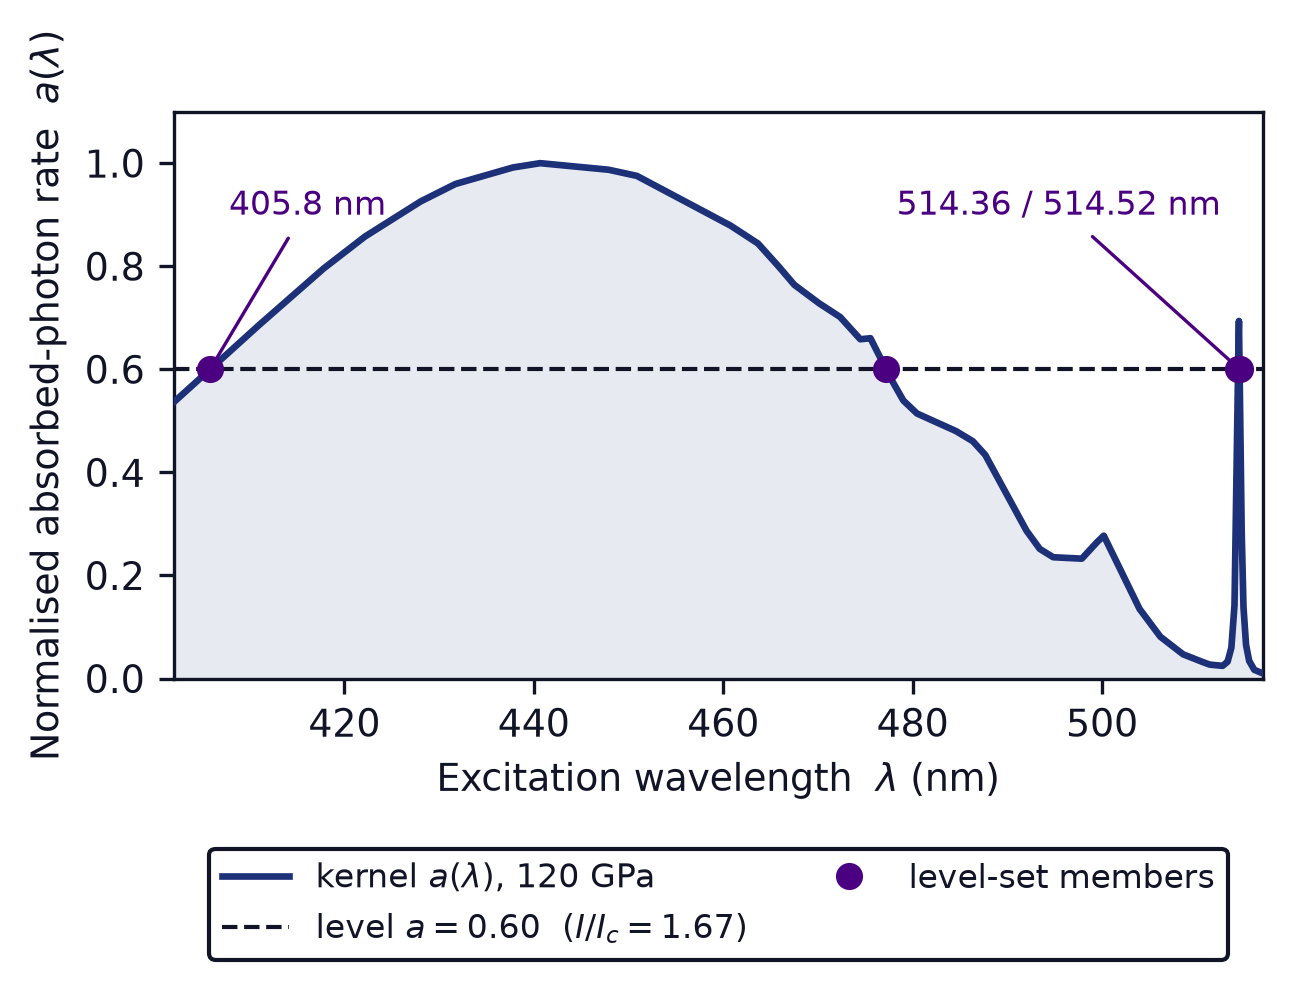
\includegraphics[width=0.58\linewidth]{image/wrn_level_set_members.png}
  \caption{Frozen v3 kernel \(a(\lambda)\) at 120 GPa, normalised to its maximum at
  440.64 nm, cut by the level \(a=0.60\) (\(I/I_c=1.67\)). The four intersections are
  the level-set members the test must compare; the two on the zero-phonon line are
  0.16 nm apart.}
  \label{fig:levelset}
\end{figure}

% =========================================================
% 4. Gap / Failure
% =========================================================
\sectionblock{Gap / Failure}

\begin{itemize}[leftmargin=8mm]
  \item The blue member exists only below \(I/I_c=1.8646\), where it reaches the 402 nm edge of the published window and leaves it. That edge is the edge of the figure, not a band edge (K1), so the member's position there is not physically anchored and the usable range of the test is \(1<I/I_c<1.86\).
  \item The two zero-phonon-line members at 514.36 and 514.52 nm are 0.16 nm apart and cannot be illuminated separately (limitation L1), so only two of the four members are accessible and the level set is not tested in full.
\end{itemize}

% =========================================================
% 5. Next Step
% =========================================================
\sectionblock{Next Step}

Collect the published wavelength dependence of the NV\(^0\)/NV\(^-\) ratio between 405 and 532 nm, derive the expected difference between the 405.8 nm and 477.2 nm members, and only then fix the measurement conditions.

% =========================================================
% 6. References
% =========================================================
\sectionblock{References}

\begin{enumerate}[leftmargin=8mm]
  \item P. Bhattacharyya, \textit{Principle and applications of quantum metrology in diamond anvil cells using the Nitrogen Vacancy color center}, PhD thesis, University of California, Berkeley (Fall 2022), pp.~65--66 and Fig.~6.2(d)(e).
  \item K. O. Ho, C. Dailledouze, V. \v{Z}alandauskas \textit{et al.}, ``Optical Stability and Photophysics of NV Centers in Diamond up to 120 GPa,'' arXiv:2606.02399v1 [quant-ph] (2026). Source of the optical kernel \(A(\lambda,P)\) that defines the level set.
\end{enumerate}

\end{document}
